%!TEX root = ../main.tex
%%%%%%%%%%%%%%%%%%%%%%%%%%%%%%%%%%
% Links:
%
% Difficulty:
% Companies: 
%%%%%%%%%%%%%%%%%%%%%%%%%%%%%%%%%%

\chapter{Generate points in circle uniformly}
\label{ch:random_points_in_circle}
\section*{Introduction}
This chapter's problem concerns uniformly generating a (potentially large) number of random points in a circle of a certain radius. Despite its simplicity the problem poses some unexpected challenges. We will discuss the best approach to this problem as well as one solution that many candidates provide which, whilst initially appearing correct actually fails in one crucial aspect (spoiler: it does not distribute points uniformly). 

\section{Problem statement}
\begin{exercise}
Write a function that, given a circle of radius $r$ and centered at $(x,y)$ where $r,x,y \in \mathcal{R}$ returns a uniformly distributed point in the circle.
\end{exercise}


\section{Clarification Questions}

\begin{QandA}
	\item \begin{questionitem} \begin{question} What exactly does it mean for the point to be uniformly distributed?  \end{question} 	 
    \begin{answered}
		\textit{It means that every point of the circle has the same probability of being picked/generated by the function}.
	\end{answered} \end{questionitem}
\end{QandA}

\section{Discussion}
\label{random_points_in_circle:sec:discussion}
Before discussing solutions it is worth mentioning that the fact that the circle is centered at $(x,y)$ makes very little difference and we can continue our discussion as if it were centered at $(0,0)$. This is the case because all the points we generate can then be translated to $(x,y)$ by simply adding $x$ and $y$ to the $x$-coordinate and $y$-coordinate of the generated point.

\subsection{Polar Coordinates - The wrong approach}
\label{random_points_in_circle:sec:buggy}
Let's start by discussing an intuituve, but ultimately incorrect, approach. One might think that in order to pick a point in the circle it is sufficient to 
\begin{enumerate}
	\item Pick a random angle $\theta \in [0, 2\pi[ $
	\item Pick a random radius $\overline{r} \in [0,r]$
	\item Generate the Cartesian coordinates of the point given the radius and the angle (polar coordinates \cite{cit:wiki:polarcoordinates}) as (see Figure \ref{fig:random_points_in_cirle:polar_coordinates}):
	\begin{gather*}
		 x=\overline{r}\sin(\theta) \\
		 y=\overline{r}\cos(\theta) 
	\end{gather*}
\end{enumerate}

\begin{figure}
	\label{fig:random_points_in_cirle:polar_coordinates}
	\centering
	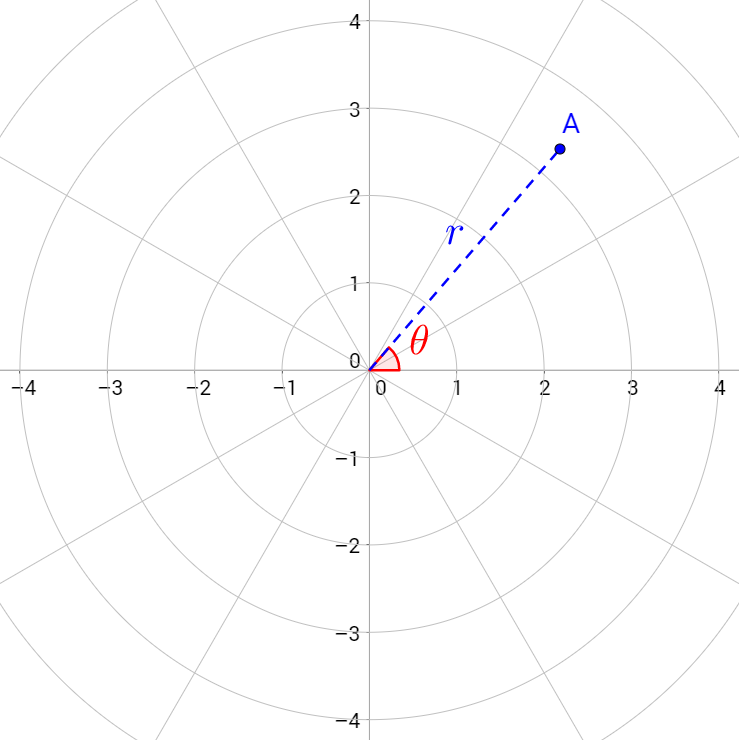
\includegraphics[scale=0.3]{sources/random_points_in_circle/images/polar-coordinate}
	\caption{Generation of a random point in polar coordinates given a random angle $\theta$ and a random radius $r$.}
\end{figure}

Unfortunately, despite its appealing simplicity, this approach is wrong as it fails to produce points that are  distributed uniformly in the circle. Before examining the mathematical proof it is instructive to have a look at Figure \ref{fig:random_points_in_cirle:buggy} which is drawing a large number of points on the circle generated using this incorrect solution. As you can see,  the points are not generated uniformly as their density is higher towards the center. 
The bottom line is, do not use this solution in an interview. A possible matlab implementation of this buggy approach is shown at [SORRY DELETED YOUR REFERENCE BY ACCIDENT]

\lstinputlisting[language=Matlab, caption=Non-uniform random point in a circle generation using Matlab,label=list:random_points_in_circle:buggy]{sources/random_points_in_circle/buggy_random_point.m}

\begin{figure}
	\label{fig:random_points_in_cirle:buggy}
	\centering
	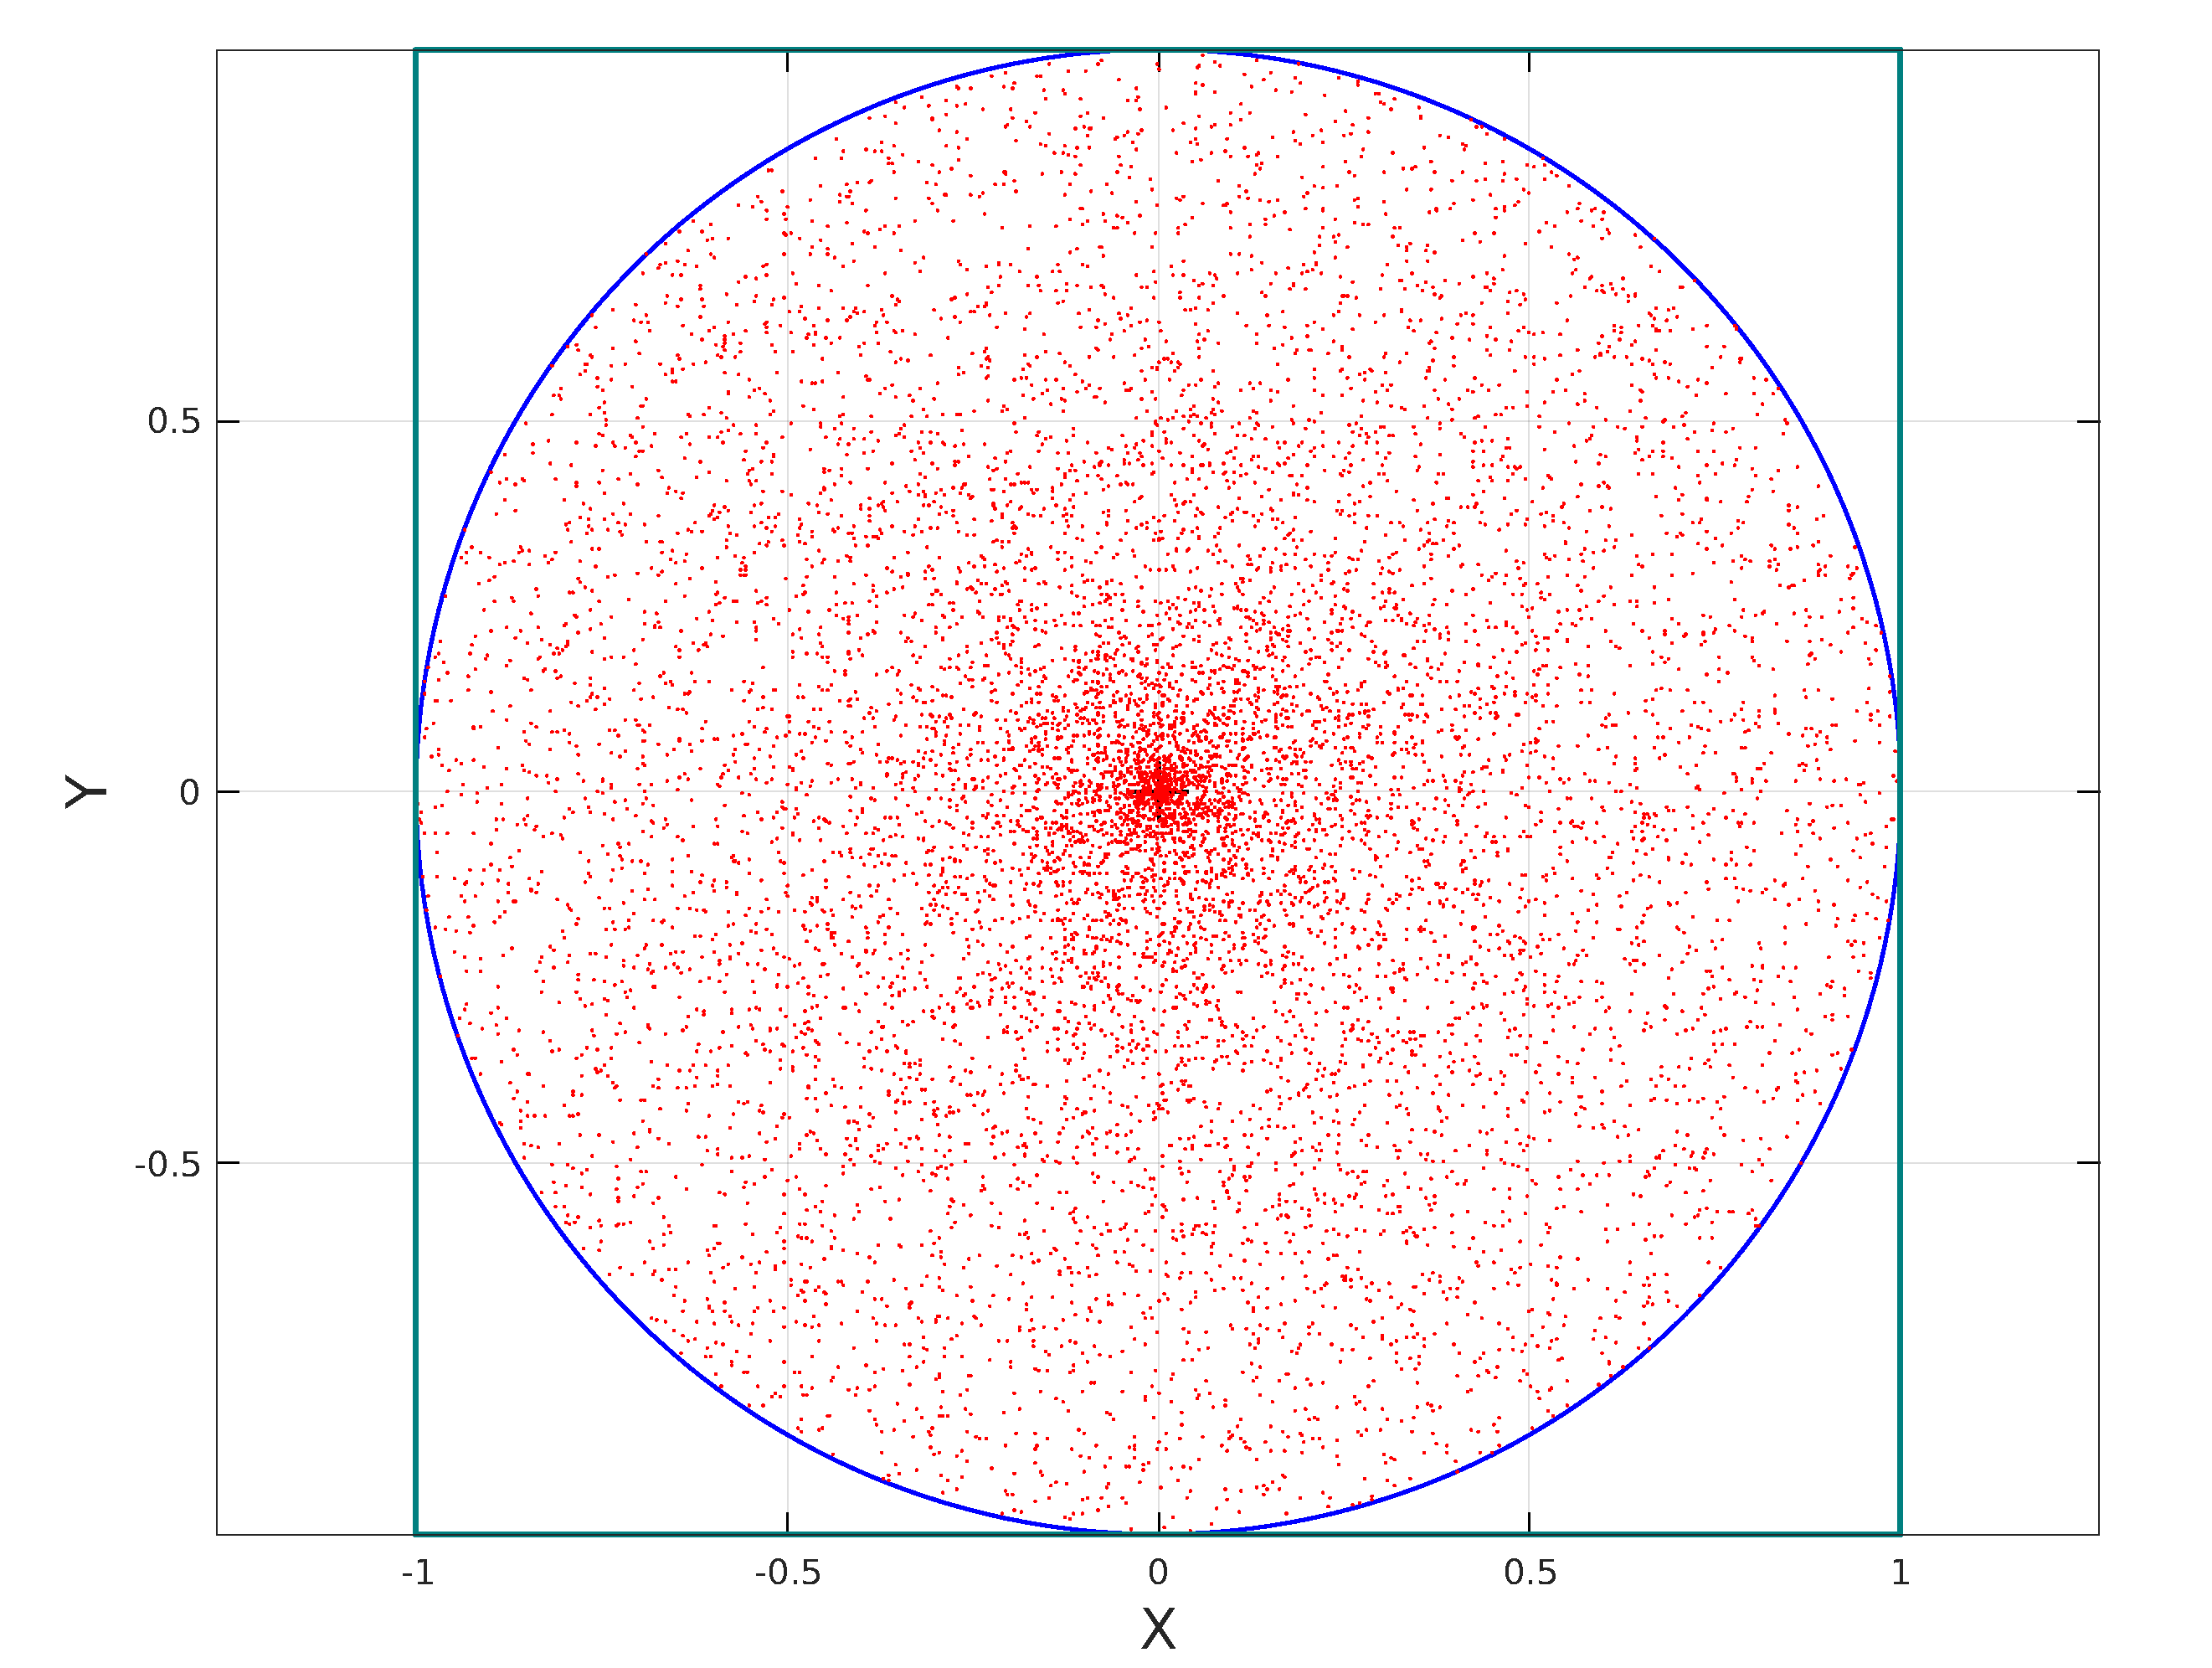
\includegraphics[scale=0.3]{sources/random_points_in_circle/images/buggy_points}
	\caption{Large number of points generated using the approach described in Section \ref{random_points_in_circle:sec:buggy}. Note that the density of points is not uniform as more points are packed around the center.}
\end{figure}

\subsection{Loop approach}
\label{random_points_in_circle:sec:loop}
A good way to ensure that the point density is uniform across on the surface of the circle is to pick a point randomly in an enclosing square and make sure that we discard all the points that lie outside the circle. In other words, we keep asking for a random point $(p_x=\text{rand()}, p_y=\text{rand()})$ in the enclosing square until the following is true: $p_x^2 + p_y^2 \leq r$. In this way we are guaranteed to generate uniformly distributed points because we pick those points from a set of points that are already uniformly distributed in a square, and we exclude those which are not inside the circle. This method is also known as the exclusion method. Figure \ref{fig:random_points_in_cirle:loop} depicts a large number of points generated with this method.

The downside here is that we might need to generate a number of points in the square before getting lucky and picking one lying in the circle. We need to make on average $\approx 1.2732$ tries before getting a point in the circle. This number is  the ratio between the are of enclosing square and the area of the enclosed circle i.e. $\frac{(2r)^2}{\pi r^2} = \frac{4}{\pi}$. 

\begin{figure}
	\label{fig:random_points_in_cirle:loop}
	\centering
	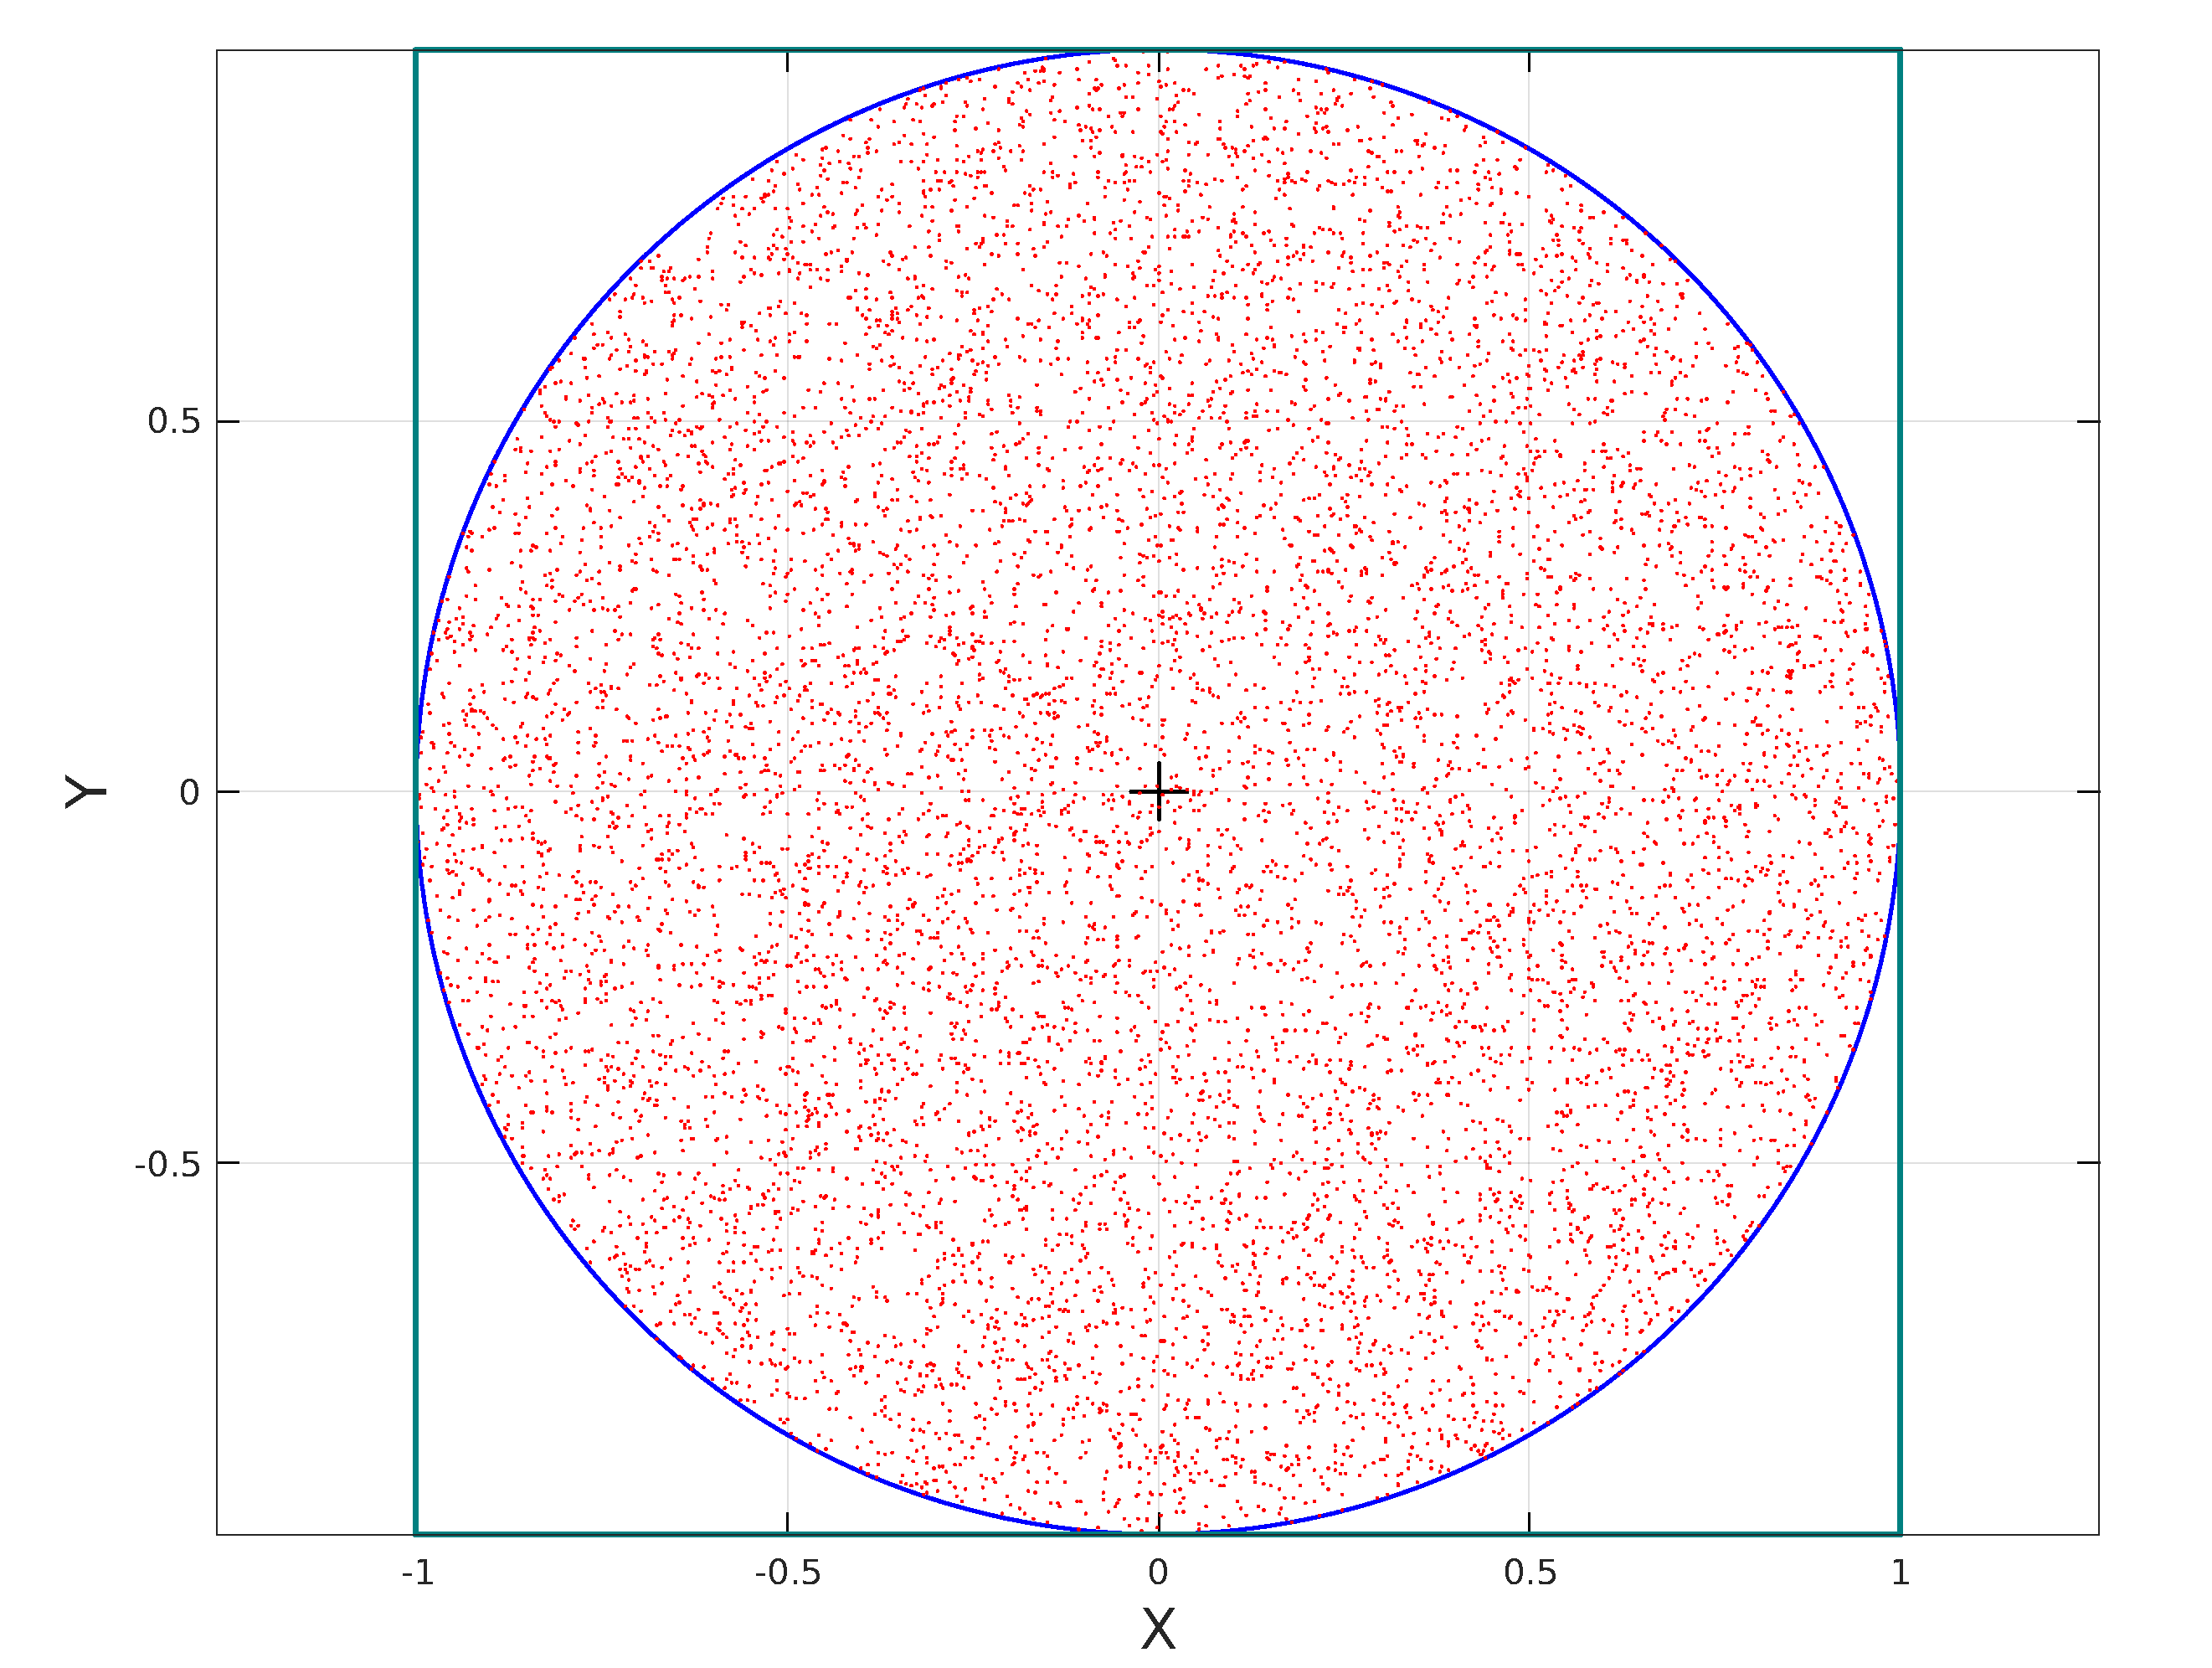
\includegraphics[scale=0.3]{sources/random_points_in_circle/images/loop_points}
	\caption{Large number of points generated using the approach described in Section \ref{random_points_in_circle:sec:loop}.}
\end{figure}

A Matlab implementation of this approach is shown in Listing \ref{list:random_points_in_circle:loop}.

\lstinputlisting[language=Matlab, caption=Random point in a circle generation using the exclusion method.,label=list:random_points_in_circle:loop]{sources/random_points_in_circle/random_point_loop.m}

\subsection{Polar Coordinates - The right approach}
\label{random_points_in_circle:sec:polar_sqrt}


In order for the points to be distributed uniformly it is necessary that the average distance between the points be the same regardless of how far they lie from the center of the circle. This means that,  looking at the points generated on a circumference of radius $2$, there have to be twice as many points as the the number of points on a circumference of radius $1$. A circumference that is twice as long translates to needing twice as many points to maintain the same density. 
Another intuitive way to understand why simply picking a random angle and a random radius is not enough would be to think about having to distribute $10$ points at random on a circle of radius $1$ and $2$. It is clear that the circumference of radius $2$ would look emptier than the one with radius $1$ simply because there is more circumference to be filled but a constant amount of points. 

The fundamental problem with the appraoch described in Section \ref{random_points_in_circle:sec:buggy} is that the area of the circle is not uniformly covered. The random radius cuts through the area of the circle and this is the only parameter that affects how the points are going to be distributed across the full area of the circle. Therefore we should focus our attention how we can pick a better radius by making sure that larger radii are picked more often to accommodate for the larger area they define. In other words, we need to ensure that our random function for picking the radius takes the area of our circle into account.

Consider the area $A$ of a circle of radius $r$ i.e.  $A = \pi r^2$. We can rearrange the formula so that $r = \sqrt{\frac{A}{\pi}}$. What this formula is really telling us is that the radius is proportional to $\sqrt{A}$. Now we have a way of choosing the radius that depends on the area of the circle. We can simply pick an area at random and then calculate the radius accordingly. This will make sure that the radius is picked taking into consideration the area of the circle. Figure \ref{fig:random_points_in_cirle:polar_sqrt} shows many points generated using this method. As you can see the points are generated uniformly across the area of the circle and the picture looks similar to Figure \ref{fig:random_points_in_cirle:loop}.

A C++ implementation of this method is shown in Listing \ref{list:random_points_in_circle:sqrtcpp}. Details on the random number generation in Modern C++ can be found in \cite{cit::std::random}.

\lstinputlisting[language=c++, caption=C++ implementation of the function for generating a random point in a circle described in Section \ref{random_points_in_circle:sec:polar_sqrt},label=list:random_points_in_circle:sqrtcpp]{sources/random_points_in_circle/random_points_in_circle_solution1.cpp}

\begin{figure}
	\label{fig:random_points_in_cirle:polar_sqrt}
	\centering
	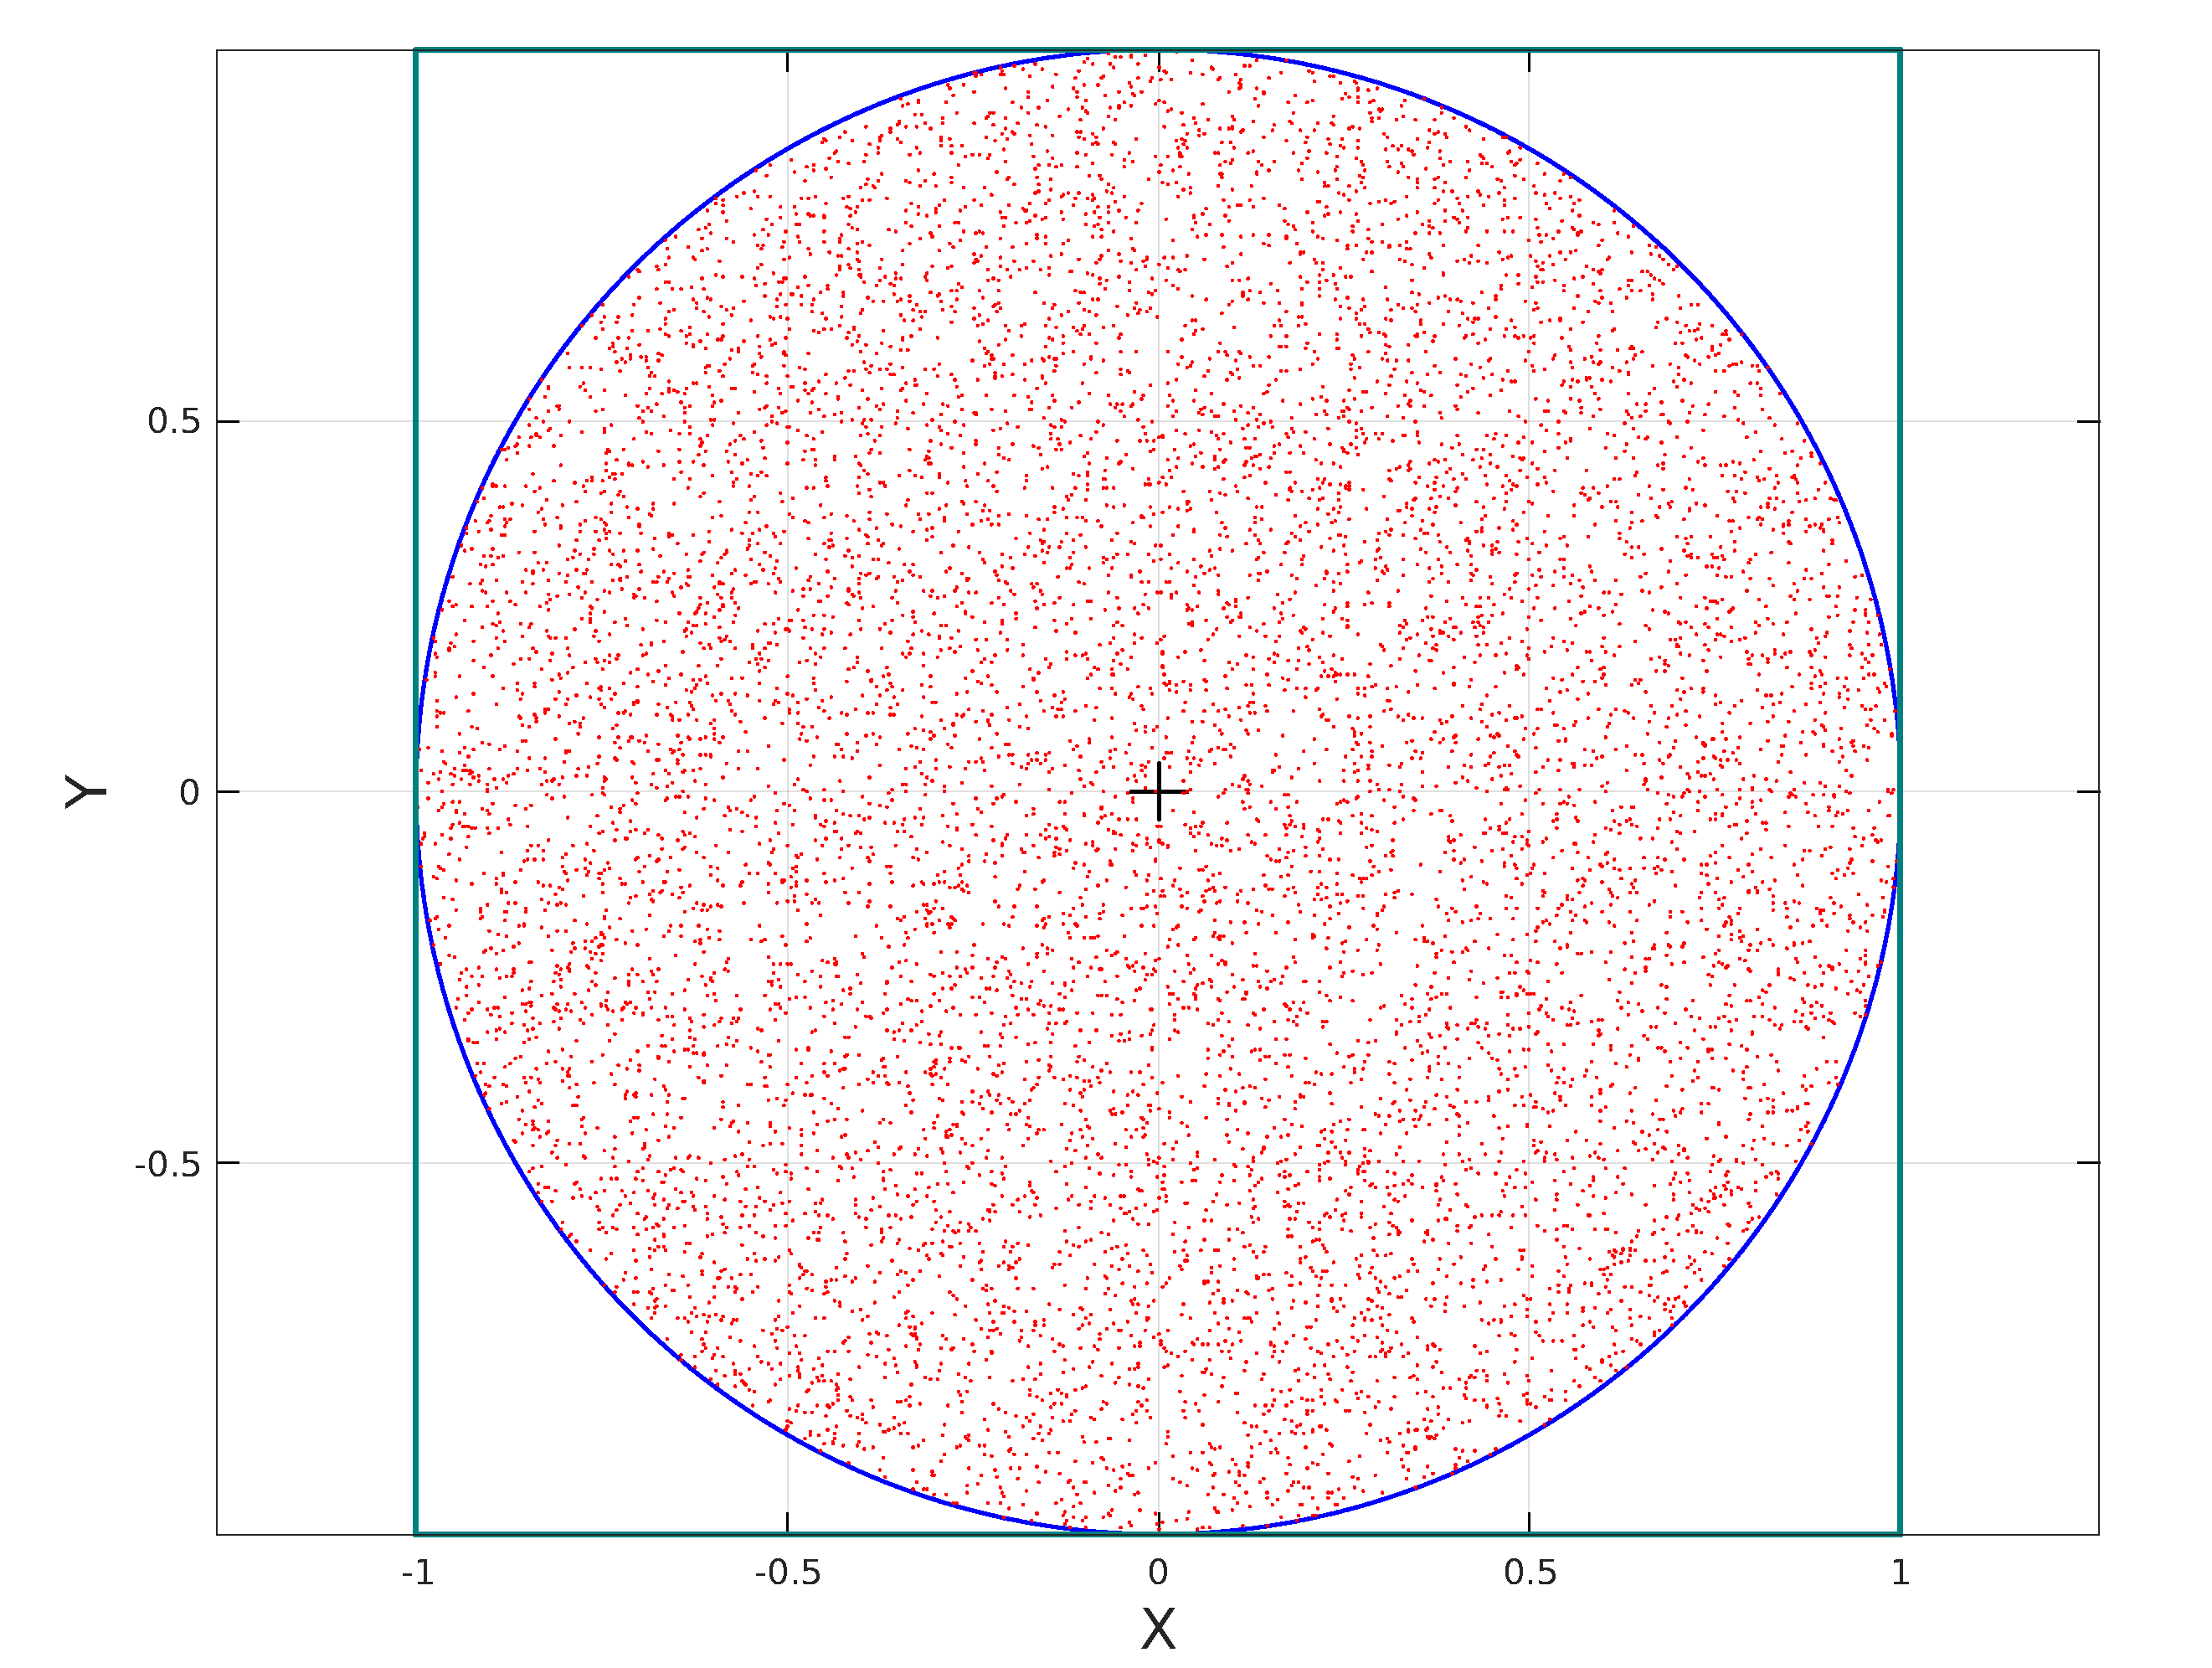
\includegraphics[scale=0.3]{sources/random_points_in_circle/images/sqrt_points}
	\caption{Large number of points generated using the approach described in Section \ref{random_points_in_circle:sec:polar_sqrt}.}
\end{figure}

A Matlab implementation of this approach is shown in Listing \ref{list:random_points_in_circle:sqrt}.

\lstinputlisting[language=Matlab, caption=Random point in a circle generation using polar coordinates and the $\approx \sqrt{A}$ dependency of the radius on the area of the circle.,label=list:random_points_in_circle:sqrt]{sources/random_points_in_circle/random_sqrt_area.m}

\subsection{Conclusion}
For both the viable methods for generating random points withing a circle which we have discussed the time and space complexity is constant although the one presented in Section \ref{random_points_in_circle:sec:polar_sqrt} will probably have better performance when included in a hot path i.e. in a loop for the generation of many random points.

All the code used to generate the Figures in this chapter is shown in Listing \ref{list:random_points_in_circle:drivercode}.


\lstinputlisting[language=Matlab, caption=Matlab driver code for the generation of all figures in Chapter \ref{ch:random_points_in_circle},label=list:random_points_in_circle:drivercode]{sources/random_points_in_circle/draw_points.m}